% Big TODOS (stretch goals):
% 1) From Certifiability to Transcribability
% 2) From Authenticated Channels to Signatures
% 3) Partial Synchrony and Eventual Liveness
% 4) Rewrite in ``Proofs and Refutation'' style
% 5) UC proofs

\section{Introduction}

A distributed ledger protocol is envisioned to play the role of a ``world computer''.
This world computer, evolving its state through State Machine Replication, ensures
execution is accurate as long as its ledger remains secure (is safe and live).
This security is guaranteed as long as some majority of validators are honest.

As multiple ledger protocols become deployed, each of them functions as its own
such ``world computer''. A natural question of recursive composability arises:
Can we use these ``world computers'' as validators to run further protocols on
top of them? For example, can we run an \emph{overlay} ledger protocol on top
of existing \emph{underlying} ledger protocols, treating the underlying ledger
protocols as \emph{computers} which take the role of a \emph{validator} in the
overlay protocol?

In this paper, we observe that many distributed systems protocols, among others
distributed ledger protocols e.g., Streamlet and HotStuff, can be run
on top of other existing long-running and battle-tested ledger \emph{underlying}
protocols such as Bitcoin, Ethereum, Cardano, and Dogecoin. The underlying protocols
play the role of always-online validators that participate in the overlay protocol's
execution. If we run a consensus protocol on top of existing consensus protocols,
we can realize a rollup, in the form of the overlay, which is securer than each
of the constituent underlying Layer-1s it is based on. For example, we can construct
a rollup that maintains security even if one of Bitcoin, Ethereum, Cardano, or Dogecoin
faces a catastrophic failure such as a persistent 51\% attack.

Our construction is quite generic.
The class of overlay protocols our system can run is not limited to consensus protocols,
but can be any distributed protocol, among others Reliable Broadcast, or a data availability
protocol, as long as it satisfies a minimal set of axioms: It must not use any
internally-generated randomness, and must be designed to work in the commonly used
\emph{authenticated channels} network model. The underlying ledger protocols must also
satisfy a minimal set of axioms which are satisfied by all popular blockchain and
related protocols today: It must realize a ledger functionality (with the ability
to \emph{write} transactions and \emph{read} sequences of transactions in the form of a ledger)
which promises to be secure; it must ascribe timestamps to each transaction on the ledger (a temporal ledger);
it must allow the recording of any arbitrary string inside a transaction (a bulletin board);
and it must support non-interactive clients (the ledgers must be \emph{transcribable}
into a string that can recover the original ledger).
The minimal set of axioms are satisfied by Bitcoin (Nakamoto), Ethereum, Cardano
(Ouroboros/Ouroboros Praos/Ouroboros Genesis), Dogecoin, Algorand, Monero, Sui
(HotStuff/Bullshark/Narwhal/Tusk), and all other distributed ledger protocols
to our knowledge. Notably, we don't require that the underlying protocols have
any smart contract support (although such support can greatly increase the efficiency
of our protocol), or that existing bridging is implemented between them (as
transcribability is enough to realize this functionality). Our construction works on
top of both proof-of-work and proof-of-stake blockchains, among others.

\noindent
\textbf{Our contributions.} The contributions of this paper are the following:

\begin{enumerate}
  \item We put forth \emph{rollerblade}, a general method that allows transforming
        distributed systems protocols from the \emph{party} to the \emph{ledger}
        setting.
  \item We show how our protocol works on top of any proof-of-work or proof-of-stake
        blockchain with minimal axiomatic assumptions. We give the exact properties
        required of the underlying ledger protocols and observe that smart contract
        capabilities and certificates are not necessary (but are helpful). Our
        protocols can run on top of Bitcoin, Ethereum, Cardano, etc.
  \item We precisely define the formulation of distributed systems protocols
        required so that they can undergo the \rollerblade transform.
  \item We prove our generic transformation always yields good results by
        using a reduction-based simulation argument connecting the
        ledger setting and the party setting. The analogies elicited through
        our transform give insights about the functionality of ledger protocols
        more broadly and may be of independent interest.
  \item We use our transform to instantiate a ledger protocol on top of
        other ledger protocols. The resulting protocol is a layer-2 rollup that
        guarantees better security than the composited layer-1s.
\end{enumerate}

% TODO: move to end of paper
\noindent
\textbf{Related work.} Building a reliable system by composing potentially faulty components
is a classical engineering problem~\cite{von1956probabilistic,moore1956reliable}.
In the era of consensus, the seminal
paper by Lamport that introduced the Byzantine Fault Tolerance problem~\cite{shostak1982byzantine}
aims to solve a reliability problem, where different processors disagree about their
outcomes. The composition of multiple \emph{blockchain} protocols was explored by
Kiayias et al.~cite{fitzi2020ledger}, but for the purpose of performance in terms of throughput
and latency, not reliability. The idea of borrowing security from one chain to
secure another was first proposed in the context of \emph{merged mining}~\cite{namecoin}, where
a strong proof-of-work blockchain secures a weaker proof-of-work blockchain. This
concept was later extended to \emph{merged staking}~\cite{pos-sidechains}, where a
strong proof-of-stake \emph{parent chain} lends its security to a less secure
\emph{child chain}. Similar ideas have recently appeared in Cosmos proof-of-stake
chains as \emph{Mesh Security}. Hybrids between different consensus mechanisms
have also been proposed. The idea of \emph{checkpointing}
one blockchain onto another to borrow security was formalized by Karakostas et al.~\cite{karakostas2021securing},
and has been applied to secure newly created proof-of-work systems using stronger
preexisting proof-of-stake systems. Such constructions are uni-directional:
one ``parent'' chain is designated as authoritative and \emph{stronger},
while the ``child'' chain is designated as \emph{weaker} and in need of securing.
The idea of composing ledgers to achieve a more reliable overlay ledger
was first proposed in a short Cosmos GitHub issue called
\emph{recursive Tendermint}~\cite{recursive-tendermint}.
This concept was expanded upon by TrustBoost~\cite{trustboost}
where they build a composition using Cosmos as the underlying
construction, IBC for cross-chain communication, and Information Theoretic
HotStuff as the overlay protocol. Regrettably, their construction is not
accompanied by a proof of security.

\noindent
\textbf{Practical efficiency.}
Our construction is about what compositions of ledgers are theoretically \emph{possible},
so we will not be concerned with the efficiency of our construction beyond the
theoretical desire to remain polynomial. Our treatment
is generic, and our aim is to formulate a minimal set of axioms
required of underlying and overlay protocols to render them composable.
Due to the generality of our construction, certain optimizations will not be
possible, but efficiency can be greatly increased for concrete underlying
protocols, for example leveraging smart contract capabilities if they are
available. For a particular example on Tendermint, see TrustBoost~\cite{trustboost}.

\begin{figure*}
    \centering
    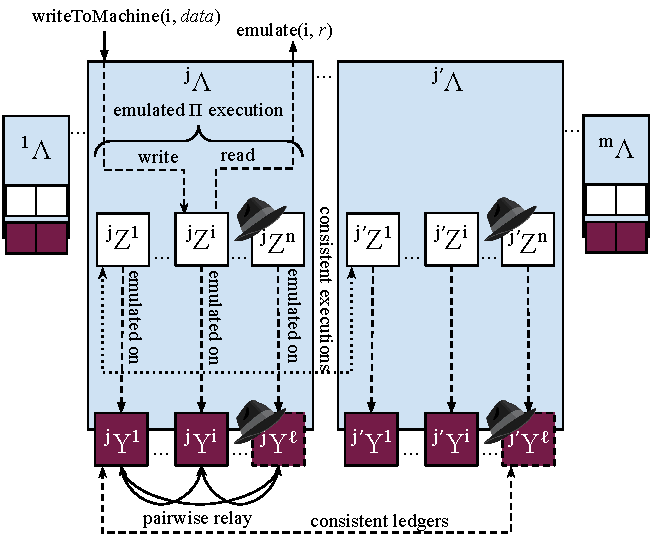
\includegraphics[width=0.9 \textwidth,keepaspectratio]{figures/rollerblade-overview.pdf}
    \caption{An overview of the \rollerblade construction.
             There are $m$ \rollerblade clients $\LLambda[1], \ldots, \LLambda[j], \ldots, \LLambda[m]$.
             Each $\LLambda[j]$ such client of them is executing $n$ instances $\Z[j][1], \ldots, \Z[j][i], \ldots, \Z[j][n]$
             of the overlay protocol $\Pi$ within it.
             To emulate the $i^\text{th}$ instance $\Z[j][i]$, the respective
             underlying protocol $\Y[j][i]$ is used.
             These underlying protocols are pairwise relayed to each other
             (shown only in $\LLambda[j]$ for clarity).
             Some of the underlying
             protocols may be rendered insecure (a black hat); their respective
             $\Z[j][i]$ instances behave dishonestly (also a black hat).
             The construction will ensure that the executions of $\Z[j][i]$ and
             $\Z[j'][i]$ are ``consistent'' if $i$ is a good underlying protocol.}
    \label{fig.rollerblade-overview}
\end{figure*}

% TODO: Rewrite the paper in Lakatos "Proofs and Refutations" format
% 1) Describe concrete protocol for overlay ledger protocols only
% 2) Describe (and break) naive construction that uses a "majority ledger" voting gate
% 3) Observe that a full consensus protocol must be run as the overlay
% 4) Describe (and break) the construction that records "netouts" on chain
% 5) Describe the full simulation-based construction
% 6) Generalize to non-ledger protocols
% 7) Generalize to transcribable protocols instead of just certifiable
\noindent
\textbf{Construction overview and paper structure.}
% Model
We begin by describing the model in Section~\ref{sec:model}, in which
we define the axioms that are required of the overlay and underlying protocols,
as well as our network and time assumptions.

% Rollerblade clients
The execution is conducted by \emph{\rollerblade clients},
the users of the overlay protocol.
Each of them operates a full node for each of the underlying ledger protocols.
Each of the \rollerblade clients simulates \emph{each} party of the overlay
ledger protocol locally, by using the respective underlying ledger protocol
as a ``guide'' to the overlay party's execution.
The respective underlying ledger indirectly records all the
user input to the overlay protocol parties, as well as the network
messages exchanged between the overlay participants.

% Writing
Any \rollerblade client can attempt to \emph{write} an input to any
of the overlay party simulations. This is performed by recording this
\emph{write instruction} to the respective underlying chain. In case
the chain written to is secure, the other \rollerblade clients will
also receive the instruction in question and replicate it within their
own simulations.

% Checkpointing
The
state of each chain is relayed to each other chain by helpful but
untrusted relayers, at least one of which is assumed to be honest
(any \rollerblade client that does not trust the relayers can relay
the data themselves). When a checkpoint of a source ledger
appears within target ledger, this corresponds to a network message
exchange from the simulated source party to the simulated target party.
Whereas no network messages are recorded on-ledger at any time,
the \rollerblade client can simulate the network messages that
\emph{would have been sent} by the source by looking at the checkpointed
source ledger data and performing a recursive simulation.
This whole construction is described in Section~\ref{sec:construction}.

% The two conjectures
Our analysis is conducted in two central lemmas: The \emph{Simulation Lemma}
and the \emph{Cross-Party Lemma}.
Firstly, the Simulation Lemma pertains to the comparison of the execution
of an overlay protocol in the ledger setting and within the confines of
\emph{one} \rollerblade client in the party setting.
It states that the execution in the ledger setting
is equivalent to some execution in the \emph{party} setting.
We prove this by a reduction-based simulation argument.
Secondly, the Cross-Party Lemma concerns the execution of \emph{multiple}
\rollerblade clients. It state that the execution of a simulated party
within one \rollerblade client is the ``same'' as the execution of the
same simulated party within a different \rollerblade client, as long
as the respective underlying ledger is secure.
None of the two lemmas require any honesty assumptions.
These lemmas are stated and proven in Section~\ref{sec:analysis}.

% The concrete consensus example
Lastly, as an example use-case, we instantiate our \rollerblade construction
to run a consensus protocol on top which allows the creation of a ``reliable
rollup'' that runs on top of multiple underlying ledgers and offers better security
than any of its constituents alone. The construction can be based on top of any
overlay consensus protocol (e.g., Streamlet or HotStuff) and uses a simple
majority voting rule.  We state and prove a security corollary
using the two lemmas as puzzle pieces, assuming secure majority of the underlying
ledgers, and that the overlay protocol is a good protocol. These results
are illustrated in Section~\ref{sec:consensus}.

% TODO: Table of analogies?

% The execution is conducted by the overlay users of the protocol.
% Each of them operates a full node for each of the underlying ledger protocols.
% When any of the overlay nodes wishes to write a transaction for
% their ledger, they replicate and post that transaction to each of
% the underlying DLPs. They then wait for the transaction to be included
% in each of the underlying DLPs, then take a majority vote among them
% to determine their own reported ledger. This construction is described
% in Section~\ref{sec:construction-naive}.
%
% Unfortunately, a simple majority vote is insufficient because each
% underlying DLP may include transactions in a different order. Hence,
% the disagreement must be solved in a fashion akin to running a BFT
% (such as \emph{Streamlet}~\cite{streamlet} or \emph{HotStuff}~\cite{hotstuff})
% protocol ``on top''. The core idea is to treat every underlying DLP
% as a \emph{participant} in the overlay BFT. The \emph{security} of
% each DLP then roughly corresponds to the \emph{honesty} of the
% respective party. Due to the security of the overlay BFT protocol
% and the fact that the majority of underlying DLPs are secure, the
% resulting ledger read from the overlay BFT will allow the overlay
% parties to reach agreement between themselves. This construction
% is described in Section~\ref{sec:construction-bft}.
%
% BFT protocols are designed to run between \emph{parties}, not DLPs.
% A translation of the BFT protocol must take place so that it can be
% utilized with DLPs as parties. This requires some technical work
% which entails swapping out any of its cryptographic signature creation
% and verification, and the removal of any non-determinism by delegating
% it to an oracle. The networking assumptions of the BFT protocol then
% must be translated to the respective DLP assumptions by treating
% network delay as ledger liveness. These \emph{virtualization} technical
% details are given in Section~\ref{sec:construction-oraclized}.
%
% Next, we show that our construction applies to a wide variety of
% protocols by discussing how it can be run on top of proof-of-work,
% proof-of-stake, and permissioned protocols. We also remove the requirement
% that any of the underlying chains require any smart contract capability,
% although smart contracts can improve our performance. These compatibility
% issues are discussed and the exact mechanism of mutual checkpointing
% that does not rely on smart contracts is discussed in
% Section~\ref{sec:compatibility}.
%
% In Section~\ref{sec:analysis} we prove that our protocol is secure by
% stating and showing a \emph{metatheorem} which, in essence, tells us that any
% party-based execution of a BFT protocol and the respective DLP-based
% execution of the same protocol suitably translated are the same. This
% then allows the translation of any existing BFT theorem (such as Streamlet's
% or HotStuff's security theorems) from the party setting to the DLP setting,
% treating both the BFT protocol on top as well as the underlying DLPs as
% black boxes following a minimal set of axioms.
